\documentclass{beamer}\usepackage[]{graphicx}\usepackage[]{color}
%% maxwidth is the original width if it is less than linewidth
%% otherwise use linewidth (to make sure the graphics do not exceed the margin)
\makeatletter
\def\maxwidth{ %
  \ifdim\Gin@nat@width>\linewidth
    \linewidth
  \else
    \Gin@nat@width
  \fi
}
\makeatother

\definecolor{fgcolor}{rgb}{0.345, 0.345, 0.345}
\newcommand{\hlnum}[1]{\textcolor[rgb]{0.686,0.059,0.569}{#1}}%
\newcommand{\hlstr}[1]{\textcolor[rgb]{0.192,0.494,0.8}{#1}}%
\newcommand{\hlcom}[1]{\textcolor[rgb]{0.678,0.584,0.686}{\textit{#1}}}%
\newcommand{\hlopt}[1]{\textcolor[rgb]{0,0,0}{#1}}%
\newcommand{\hlstd}[1]{\textcolor[rgb]{0.345,0.345,0.345}{#1}}%
\newcommand{\hlkwa}[1]{\textcolor[rgb]{0.161,0.373,0.58}{\textbf{#1}}}%
\newcommand{\hlkwb}[1]{\textcolor[rgb]{0.69,0.353,0.396}{#1}}%
\newcommand{\hlkwc}[1]{\textcolor[rgb]{0.333,0.667,0.333}{#1}}%
\newcommand{\hlkwd}[1]{\textcolor[rgb]{0.737,0.353,0.396}{\textbf{#1}}}%
\let\hlipl\hlkwb

\usepackage{framed}
\makeatletter
\newenvironment{kframe}{%
 \def\at@end@of@kframe{}%
 \ifinner\ifhmode%
  \def\at@end@of@kframe{\end{minipage}}%
  \begin{minipage}{\columnwidth}%
 \fi\fi%
 \def\FrameCommand##1{\hskip\@totalleftmargin \hskip-\fboxsep
 \colorbox{shadecolor}{##1}\hskip-\fboxsep
     % There is no \\@totalrightmargin, so:
     \hskip-\linewidth \hskip-\@totalleftmargin \hskip\columnwidth}%
 \MakeFramed {\advance\hsize-\width
   \@totalleftmargin\z@ \linewidth\hsize
   \@setminipage}}%
 {\par\unskip\endMakeFramed%
 \at@end@of@kframe}
\makeatother

\definecolor{shadecolor}{rgb}{.97, .97, .97}
\definecolor{messagecolor}{rgb}{0, 0, 0}
\definecolor{warningcolor}{rgb}{1, 0, 1}
\definecolor{errorcolor}{rgb}{1, 0, 0}
\newenvironment{knitrout}{}{} % an empty environment to be redefined in TeX

\usepackage{alltt}

\usepackage{default}
\usepackage{animate} %need the animate.sty file 
\usepackage{graphicx}
%\graphicspath{{/home/sahir/Dropbox/jobs/laval/minicours/slides/}}
\usepackage{hyperref, url}
%\usepackage[round,sort]{natbib}   % bibliography omit 'round' option if you prefer square brackets
%\bibliographystyle{apalike}
\usepackage{biblatex}
\bibliography{bib.bib}
% Removes icon in bibliography
\setbeamertemplate{bibliography item}[text]

\usepackage[figurename=Fig.]{caption}
\usepackage{subfig}
\usepackage{tikz, pgfplots}
\usetikzlibrary{arrows,shapes.geometric}
\usepackage{color, colortbl,xcolor}
\definecolor{lightgray}{RGB}{200,200,200}
\definecolor{myblue}{RGB}{0,89,179}
\usepackage{comment}
\setbeamercolor{frametitle}{fg=myblue}
\setbeamercolor{section in head/foot}{bg=myblue, fg=white}
\setbeamercolor{author in head/foot}{bg=myblue}
\setbeamercolor{date in head/foot}{bg=myblue}

\usepackage{array}
\newcolumntype{L}{>{\centering\arraybackslash}m{3cm}} % used for text wrapping in ctable
\usepackage{ctable}
\usepackage[utf8]{inputenc}
\usepackage{fontenc}
\usepackage{pifont}% http://ctan.org/pkg/pifont
\newcommand{\cmark}{\ding{51}}%
\newcommand{\xmark}{\ding{55}}%
\def\widebar#1{\overline{#1}}
\definecolor{whitesmoke}{rgb}{0.96, 0.96, 0.96}

\usepackage{fontspec}
%\setsansfont{Fira Sans}
%\setmonofont{Fira Mono}
\setsansfont[ItalicFont={Fira Sans Light Italic},BoldFont={Fira Sans},BoldItalicFont={Fira Sans Italic}]{Fira Sans Light}
\setmonofont[BoldFont={Fira Mono Medium}]{Fira Mono}


\setbeamercolor{itemize item}{fg=myblue}
\setbeamertemplate{itemize item}[square]

\setbeamertemplate{navigation symbols}{\usebeamercolor[fg]{title in head/foot}\usebeamerfont{title in head/foot}\insertframenumber}
\setbeamertemplate{footline}{}

\newtheorem{proposition}[theorem]{Proposition}
\newtheorem{exercise}[theorem]{Exercise}

\titlegraphic{\hfill
\includegraphics[height=1cm]{mcgill_logo.png}}


%% You also use hyperref, and pick colors 
\hypersetup{colorlinks,citecolor=orange,filecolor=red,linkcolor=brown,urlcolor=blue}

\newcommand {\framedgraphiccaption}[2] {
	\begin{figure}
		\centering
		\includegraphics[width=\textwidth,height=0.8\textheight,keepaspectratio]{#1}
		\caption{#2}
	\end{figure}
}

\newcommand {\framedgraphic}[1] {
	\begin{figure}
		\centering
		\includegraphics[width=\textwidth,height=0.9\textheight,keepaspectratio]{#1}
	\end{figure}
}


\AtBeginSection[]{
	\begin{frame}
		\vfill
		\centering
		\begin{beamercolorbox}[sep=8pt,center,shadow=true,rounded=true]{title}
			\usebeamerfont{title}\insertsectionhead\par%
		\end{beamercolorbox}
		\vfill
	\end{frame}
}

\newcommand\Wider[2][3em]{%
	\makebox[\linewidth][c]{%
		\begin{minipage}{\dimexpr\textwidth+#1\relax}
			\raggedright#2
		\end{minipage}%
	}%
}
\IfFileExists{upquote.sty}{\usepackage{upquote}}{}
\begin{document}
%\sffamily



\title{Introduction to Regression Trees}
%\author{Sahir Bhatnagar \inst{1}}
\author[shortname]{Sahir Rai Bhatnagar, PhD Candidate (Biostatistics) }
\institute[shortinst]{Department of Epidemiology, Biostatistics and Occupational Health}

\title{Sampling Distributions (EPIB 607)}
\author{Sahir Bhatnagar and James Hanley}
\institute{
	Department of Epidemiology, Biostatistics, and Occupational Health\\
	McGill University\\
	
	\vspace{0.1 in}
	
	\texttt{sahir.bhatnagar@mcgill.ca}\\
	\texttt{\url{https://sahirbhatnagar.com/EPIB607/}}}

%\date

\maketitle

\section{Parameters,  Samples,  and  Statistics}

\begin{frame}{Parameters,  Samples,  and  Statistics}
\begin{itemize}
		\item \textbf{Paramter}: An  unknown  numerical  constant  pertaining  to  a  population/universe,  or  in  a  statistical  model. 
		\begin{itemize}
			\item $\mu$: population mean $\qquad\qquad$ $\pi$: population proportion
		\end{itemize}
	\pause
		\item \textbf{Statistic}: A  numerical  quantity  calculated  from  a  sample. The  empirical counterpart of the parameter,  used  to  \textit{estimate}  it.
		\pause
			\begin{itemize}
			\item $\bar{y}$: sample mean $\qquad\qquad$ $p$: sample proportion
		\end{itemize}
\end{itemize}

\pause
\Wider[4em]{
	\centering
	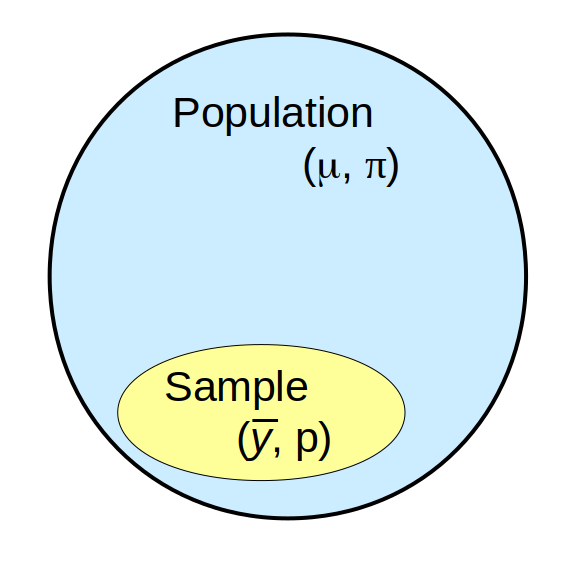
\includegraphics[scale=0.35]{MeansFig1.png}
}




\end{frame}


\begin{frame}{Examples}
\textbf{Proportions}:
	\begin{itemize}
	  \setlength\itemsep{1.2em}
	  \item Proportion of  Earth's  surface  covered  by  water
	  \item Proportion  who saw a medical doctor last year
	  \item Proportion of Québécois who don't have a family doctor
		\end{itemize}  
\pause 
	\vspace{0.1 in}
	
\textbf{Means}:
\begin{itemize}	 
	  \setlength\itemsep{1.2em} 
		\item Mean  depth  in $n$ randomly  selected  ocean  locations
		\item Mean  household  size  in $n$ randomly  selected  households.  
		\item Median  number  of  persons  under-5  in  a  sample  of $n$ households
	\end{itemize}  

\end{frame}

\frame{\frametitle{Samples must be random} 
	
\begin{itemize}
	\item 	The validity of inference will depend on the
	way that the sample was collected. If a sample was collected badly, no amount of
	statistical sophistication can rescue the study. \\ \ \\ \pause
	
	\item Samples should be \textbf{random}. That is, there should be no systematic set of
	characteristics that is related to the scientific question of interest that causes some
	people to be more likely to be sampled than others. The simplest type of randomization
	selects members from the population with equal probability (a uniform distribution). \\ \
	\\ \pause
	
	\item When conducting a study, it is always better to seek statistical
	advice sooner rather than later. Get a statistician involved at the
	\textit{planning} stage of the study... by the analysis stage, it
	may be too late!
\end{itemize}
}


\frame{\frametitle{Samples must be random - No cheating!} 
	
	\textbf{Do not cheat by} \pause 
	\begin{itemize}
		\item 	Taking 5 people from the \emph{same} household to estimate
		
		 \begin{itemize}
		 	\item proportion of Québécois who don't have a family doctor
		 	\item who saw a medical doctor last year
		 	\item average rent
		 \end{itemize}  
	 
	 \pause
	 	\vspace{0.2 in}
		
		\item Sampling the depth of the ocean \emph{only around Montreal} to estimate \begin{itemize}
			\item proportion of  Earth's  surface  covered  by  water
		\end{itemize} 

	\end{itemize}
}



\frame{\frametitle{Collecting data takes effort} 
	
	\textbf{In general} 
	\begin{itemize}
		\item The larger the sample $\to $ the more accurate the estimate (if sampling is done correctly) \pause
		
		
	\end{itemize}	
		
			 	\vspace{0.2 in}
			 	
			 		\textbf{CAVEAT} 
			 	\begin{itemize}
			 		\item Collecting more data takes effort and money!
			 		\item We will also soon discover the curse of the $\sqrt{n}$ 			 		
			 	\end{itemize}	

}


\frame{\frametitle{Collecting data takes effort} 
	
	\textbf{In general} 
	\begin{itemize}
		\item The larger the sample $\to $ the more accurate the estimate (if sampling is done correctly) \pause
		
		
	\end{itemize}	
	
	\vspace{0.2 in}
	
	\textbf{CAVEAT} 
	\begin{itemize}
		\item Collecting more data takes effort and money!
		\item We will also soon discover the curse of the $\sqrt{n}$ 			 		
	\end{itemize}	
	
}



\section{Sampling Distributions}


\frame{\frametitle{Sampling Distributions} 
	
	\begin{itemize}
				  \setlength\itemsep{2em} 
		\item Given a sample of $n$ observations from a population, we will be
		calculating estimates of the population mean, proportion, standard
		deviation, and various other population characteristics
		(parameters) \pause
		
	\item Prior to obtaining data, there is uncertainty as to which of all
		possible samples will occur \pause

\item  Because of this, estimates such as $\bar{y}$ (the sample mean) will vary
		from one sample to another
		
		
	\end{itemize}	

	
}


\frame{\frametitle{Sampling Distributions} 
	
	\begin{itemize}
		\setlength\itemsep{2em} 
		\item The behavior of such estimates in many samples of equal size is
		described by what are called \textbf{sampling distributions} \pause
		
		\item B\&M definition: The  sampling  distribution  of  a  statistic  is  the  distribution  of  values taken  by  the  statistic  in  all  possible  samples  of  the  same  size  from  the  same population.		
		
	\end{itemize}	
	
	
}

\frame{\frametitle{Why are sampling distributions important?} 
	
	\begin{itemize}
		\setlength\itemsep{2em} 
		\item They  tell  us  how  far  from  the  target  (true  value  of  the  parameter)  our  statistical  \emph{shot}  at  it  (i.e.  the  statistic  calculated  form  a  sample)  is  likely  to  be,  or, to  have  been.  \pause 
		
		\item Thus,  they  are  used  in  confidence  intervals  for  parameters. Specific  sampling  distributions  (based  on  a null value  for  the  parameter)  are also  used  in  statistical  tests  of  hypotheses.
		
	\end{itemize}	
	
	
}


\frame{\frametitle{Exercise 1: How Deep is the Ocean?} 
	
	\begin{itemize}
		\setlength\itemsep{2em} 
		\item We will get a sense of what a sampling distribution is in Exercise 1 \pause
		
		\item \textbf{CAVEAT}: This is a luxury using a toy example. In actual studies, we only get one shot!
		
	\end{itemize}	
	
	
}


\end{document}



\begin{frame}[fragile]{Collecting data takes effort}

\begin{comment}

\Wider[9em]{
	\begin{figure}
		\begin{minipage}[h]{0.49\linewidth}
			\centering
			\includegraphics[scale=0.4]{cart_pruned-crop.pdf}
			\caption{Regression}
			\label{fig:a}
		\end{minipage}
		%\hspace{0.5cm}
		\begin{minipage}[h]{0.49\linewidth}
			\centering
			\includegraphics[scale=0.20]{class_tree-crop.pdf}
			\caption{Classification}
			\label{fig:b}
		\end{minipage}
	\end{figure}
}
\end{comment}


\begin{itemize}
	\item Today's class $\to$ regression
\end{itemize}

\end{frame}







\begin{frame}{How does CART work?}
	
	Roughly speaking, there are two steps~\cite{james2013introduction}:
	\pause 
	
	\begin{enumerate}
		\setlength\itemsep{1em}
		%\item Un arbre de régression et de classification se construit de manière itérative, en découpant à chaque étape la population en deux sousensembles\nocite{lopez2015arbres}
		%\item Le découpage s’effectue suivant des règles simples portant sur les variables	explicatives, en déterminant la règle optimalequi permet de construire deux populations les	plus différenciées en termes de valeurs de la variable à expliquer
		\item We divide the predictor space - that is, the set of possible values for
		$X_1, X_2,\ldots, X_p$, into $J$ non-overlapping and exhaustive regions,
		$R_1, R_2,\ldots, R_J$.
		\item For every observation that falls into the region $R_j$, we make the same
		prediction, which is simply the mean of the response values for the
		training observations in $R_j$.
	\end{enumerate}
\end{frame}







\begin{frame}{And if we continue...}

gdsgs

%\framedgraphic{area5.pdf}

\end{frame}

\begin{frame}{Stop if the number of observations is less than 20}

gsd

%\Wider[4em]{
%\includegraphics[scale=0.45]{tree5.pdf}
%}

\end{frame}


\section{The Details}


\begin{frame}{The Details}
	
The CART algorithm requires 3 components:

\begin{enumerate}
		  \setlength\itemsep{1.5em}
	\item Defining a criterion to select the best partition among all predictors.
	\item A rule to decide when a node is terminal, i.e., it becomes a leaf.
	\item Pruning the tree to avoid over-fitting.
\end{enumerate}

\end{frame}


\begin{frame}{1. Selecting the Best Partition}
	The objective is the find the regions $R_1, \ldots, R_J$ that minimize the squared error loss:
		
	\begin{equation}
		\sum_{j=1}^{J} \sum_{i \in R_j}(y_i - \hat{y}_{R_j})^2 \label{eq:obj1}
	\end{equation}
	
	\begin{itemize}
		\setlength\itemsep{1.5em}
		\item $\hat{y}_{R_j}$: the mean response for the training observations within the
		$j$th box \pause
		\item Finding the solution to~\eqref{eq:obj1} is computationally infeasible (\textit{NP-hard}). Why? 
	\end{itemize}
	
	
\end{frame}




\section{Comparison with a Linear Model}

\begin{frame}{Comparison: Linear Model vs. CART}
\vspace*{-0.25cm}

\ctable[pos=h!,doinside=\footnotesize]{lcc}{\tnote{\cmark: yes, \xmark: no}
}{
\FL
\textbf{Characteristic\tmark} & \textbf{\texttt{Linear Model}}   & \textbf{\texttt{CART}} \ML
\rowcolor{whitesmoke}
Linearity Assumption & \cmark &    \xmark    \\
& &  \\
Distributional Assumptions & \cmark & \xmark \\
& &  \\
\rowcolor{whitesmoke}
Robust to multicollinearity &  \xmark  &  \cmark   \\ 
%& &  \\
%High-dimensional data ($n << p$) & \xmark   & \cmark     \\
& &  \\
\rowcolor{whitesmoke}
Handles complex interactions &  \xmark  &  \cmark    \\
& &  \\
%Valeurs aberrantes  &    &      \\
\rowcolor{whitesmoke} 
Allows for missing data  & \xmark   &  \cmark    \\
& &  \\
Confidence Intervals, $p$-values & \cmark & \xmark \LL
}
\end{frame}




\begin{frame}[fragile]{Linear Model}
\begin{knitrout}\scriptsize
\definecolor{shadecolor}{rgb}{0.969, 0.969, 0.969}\color{fgcolor}\begin{kframe}
\begin{alltt}
\hlkwd{lm}\hlstd{(Salary} \hlopt{~} \hlstd{Years} \hlopt{*} \hlstd{Hits,} \hlkwc{data} \hlstd{= Hitters)}
\end{alltt}
\end{kframe}
\end{knitrout}


\end{frame}





\begin{frame}[allowframebreaks]
%\nocite{breiman1984classification}
	\nocite{friedman2001elements}
	\nocite{james2013introduction}
	\nocite{lopez2015arbres}
	\frametitle{References}
\printbibliography
\end{frame}


\begin{frame}[fragile]{Session Info}
	\tiny
	
\begin{knitrout}\tiny
\definecolor{shadecolor}{rgb}{0.969, 0.969, 0.969}\color{fgcolor}\begin{kframe}
\begin{verbatim}
R version 3.5.1 (2018-07-02)
Platform: x86_64-pc-linux-gnu (64-bit)
Running under: Ubuntu 18.04 LTS

Matrix products: default
BLAS: /usr/lib/x86_64-linux-gnu/openblas/libblas.so.3
LAPACK: /usr/lib/x86_64-linux-gnu/libopenblasp-r0.2.20.so

attached base packages:
[1] stats     graphics  grDevices utils     datasets  methods   base     

other attached packages:
[1] knitr_1.20

loaded via a namespace (and not attached):
[1] compiler_3.5.1 magrittr_1.5   tools_3.5.1    stringi_1.2.4 
[5] highr_0.7      digest_0.6.16  stringr_1.3.1  pacman_0.4.6  
[9] evaluate_0.11 
\end{verbatim}
\end{kframe}
\end{knitrout}

\end{frame}

\end{document}
